%%% LaTeX Template: Designer's CV
%%%
%%% Source: http://www.howtotex.com/
%%% Feel free to distribute this template, but please keep the referal to HowToTeX.com.
%%% Date: March 2012


%%%%%%%%%%%%%%%%%%%%%%%%%%%%%%%%%%%%%
% Document properties and packages
%%%%%%%%%%%%%%%%%%%%%%%%%%%%%%%%%%%%%
\documentclass[a4paper,12pt,final]{memoir}

% misc
\renewcommand{\familydefault}{bch}	% font
\pagestyle{empty}					% no pagenumbering
\setlength{\parindent}{0pt}			% no paragraph indentation


% required packages (add your own)
\usepackage{flowfram}										% column layout
\usepackage[top=1cm,left=0.2cm,right=1cm,bottom=0.8cm]{geometry}% margins
\usepackage{graphicx}
\usepackage{epstopdf} 									% figures
\usepackage{url}											% URLs
\usepackage[usenames,dvipsnames]{xcolor}					% color
\usepackage{multicol}										% columns env.
	\setlength{\multicolsep}{1pt}
\usepackage{paralist}										% compact lists
\usepackage{tikz}
\usepackage{textcomp}

%\usepackage{anyfontsize}
\usepackage[hidelinks]{hyperref}

%%%%%%%%%%%%%%%%%%%%%%%%%%%%%%%%%%%%%
% Create column layout
%%%%%%%%%%%%%%%%%%%%%%%%%%%%%%%%%%%%%
% define length commands
\setlength{\vcolumnsep}{\baselineskip}
\setlength{\columnsep}{\vcolumnsep}

% frame setup (flowfram package)
% left frame
\newflowframe{0.265\textwidth}{\textheight}{0pt}{0pt}[left]
	\newlength{\LeftMainSep}
	\setlength{\LeftMainSep}{0.2\textwidth}
	\addtolength{\LeftMainSep}{4\columnsep}

% right frame
\newflowframe{0.7\textwidth}{\textheight}{\LeftMainSep}{0pt}[main01]

% horizontal rule between frames (using TikZ)
\renewcommand{\ffvrule}[3]{%
\hfill
\tikz{\draw[loosely dotted,color=Plum,line width=1.5pt,yshift=-#1](0, 0) -- (0pt,#3);}
\hfill\mbox{}}
\insertvrule{flow}{1}{flow}{2}


%%%%%%%%%%%%%%%%%%%%%%%%%%%%%%%%%%%%%
% define macros (for convience)
%%%%%%%%%%%%%%%%%%%%%%%%%%%%%%%%%%%%%
\newcommand{\Sep}{\vspace{1.5em}}
\newcommand{\SmallSep}{\vspace{0.5em}}

\newenvironment{Objective}
	{\ignorespaces\textbf{\color{Plum} Objective}}
	{\Sep\ignorespacesafterend}
	
\newcommand{\CVSection}[1]
	{\Large\textbf{#1}\par
	\SmallSep\normalsize\normalfont}

\newcommand{\CVItem}[1]
	{\textbf{\color{Plum} #1}}

%\urlstyle{}

%%%%%%%%%%%%%%%%%%%%%%%%%%%%%%%%%%%%%
% Begin document
%%%%%%%%%%%%%%%%%%%%%%%%%%%%%%%%%%%%%
\begin{document}

% Left frame
%%%%%%%%%%%%%%%%%%%%
%\begin{figure} 
%	\hfill
%	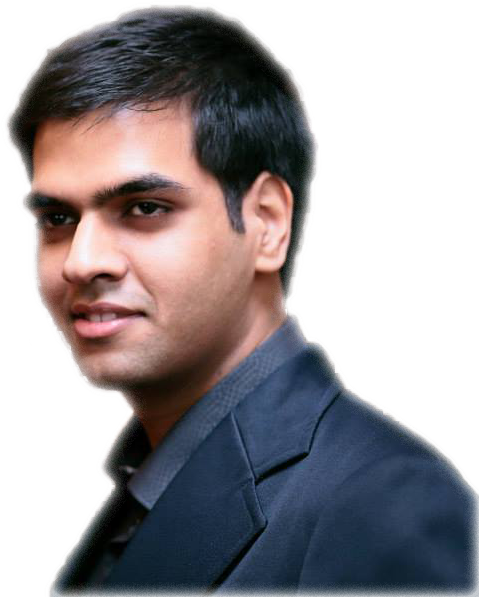
\includegraphics[width=0.8\columnwidth]{kkk}
%	\vspace{-5cm}
%\end{figure}

\begin{flushright} 
	\footnotesize
	\SmallSep
	{\bfseries{\color{Plum}{Address}}}\\
	
	Flat No.8, Katara Mansion\\
	Dr. Annie Besant Rd., Worli\\
	Mumbai - 400018, India\\
	\Sep
	{\bfseries{\color{Plum}{EMail}}}\\
	\href{mailto:vicky.p.katara@gmail.com}{vicky.p.katara@gmail.com}\\
	\Sep
	{\bfseries{\color{Plum}{Cellphone}}}\\
	\href{tel:+919867728292}{+91 986 772 8292}\\
	\Sep
		{\bfseries{\color{Plum}{Website}}}\\
	\href{http://vickykatara.orgfree.com/}{vickykatara.orgfree.com}\\
\end{flushright}\normalsize
%\begin{figure}
	%\hfill
	%\vspace{-0.3cm}
	\hspace{0.5cm}
	\vspace{-0.35cm}
	\bfseries{\color{Plum}{Contact Information}}\\\\
	\vspace{-0.1cm}
	\hspace{-0.4cm}
	
\includegraphics[width=0.8\columnwidth]{qrcode_2.eps}
%\end{figure}
\framebreak

% Right frame
%%%%%%%%%%%%%%%%%%%%
\Huge\bfseries {\color{Plum} Vicky Katara} \\
\Large\bfseries  Computer Engineering Graduate \\

\normalsize\normalfont

% About me
\begin{Objective}
\\Achieve excellence in the field of Computer Science through a Graduate course, while refining the \allowbreak ability of visualization and rationality of thought
\end{Objective}

% Education
\CVSection{Education}
\CVItem{2009 - 2013, B.E.(Computer Engineering), University of \allowbreak  Mumbai} \\
Four year undergraduate course primarily focused on Computer Science.
\SmallSep\\
{\footnotesize 
	\begin{minipage}{14cm}
		\begin{compactitem}[\color{Plum}$\circ$]
				\item Majored in Computer Software. Minored in Computer Hardware / Electronics
				\item Courses taken include:
					{\scriptsize 
							\begin{multicols}{2}
							\begin{compactitem}[\color{Plum}$\triangleright$]
									\item Computer Programming
									\item Algorithms and Data Structures
									\item Computer Networks
									\item Database Management Systems
									\item Theory of Computer Science
									\item Operating Systems 
									\item Computer Graphics
									\item Distributed Systems \& System Security
									\item Human Computer Interaction
									\item Soft Computing
									\item Image Processing
									\item \ldots
							\end{compactitem}
						\end{multicols}
					}
					\SmallSep
				\item The Degree course included a Research / Thesis topic in the Final Year.
				\item Passed out with 72.46\% with Overall Distinction. Ranked 6 out of 130 peers.
		\end{compactitem}
	\end{minipage}
	}
\SmallSep

\CVItem{2007 - 2010, Kishinchand Chellaram College}\\
Majored in Science. Consistently stood in the first 5 ranks. Took up \allowbreak vocational subject of Electrical Maintenance
\SmallSep

% Experience
\CVSection{Work Experience}
\CVItem{Jan 2014 \textendash \space present, Technology Analyst, Deloitte Consulting}\\
\SmallSep
Information Management: Business Intelligence - Data Warehousing\\
\begin{minipage}{13cm}
\begin{compactitem}[\color{Plum}$\circ$]
	{\footnotesize
		\item Recruited from Campus. Trained in Data Warehousing technologies particularly the Informatica platform
		\item Worked on short term Data Integration project for one of the leading visualization software companies in the world
		\item Currently working on a long term Enterprise Data Warehouse design and build project for one of the largest telecom service providers in the United States
		\item Working on numerous firm and community improvement initiatives
		\item Scored highest grade in Deloitte's Communication Excellence Assessment
		\item Received numerous awards and accolades
		\item Worked on massively scaled integration service deployed over a Hadoop cluster
}
\end{compactitem}
\end{minipage}
\SmallSep\\
\CVItem{May 2006 \textendash \space present, Personal Tutor}\\
\SmallSep
Part time personal tutor to high school students\\
\begin{minipage}{13cm}
	\begin{compactitem}[\color{Plum}$\circ$]
		{\footnotesize
			\item Have taught more than 20 students, all between the ages of 14 and 19
			\item Subjects taught primarily include Mathematics and Physics}
	\end{compactitem}
\end{minipage}
\SmallSep

% Projects - Start
\CVSection{Projects}
%Project-1 Start
\CVItem{Design and Development of Enterprise Data Warehouse, Telecom Client}\SmallSep\\
\begin{minipage}{13cm}
	\begin{compactitem}[\color{Plum}$\circ$]
		{\footnotesize
			\item \emph{Technical Environment:} Informatica PowerCenter and Oracle PL/SQL
			\item \emph{Industry:} Telecommunication
			\item \emph{Role:} Enterprise Data Warehouse(EDW) Designer and Developer, EDW Tester
			\item \emph{Team Size:} 11
			\item \emph{Description:} As part of this team, I designed parts of the Dimension model as a Star Constellation. The development team, of which I was a part, helped develop Informatica Mappings and associated Workflows to perform the Extract, Transform and Load process to populate the data warehouse. I was also part of the Enterprise Data Warehouse testing team which validated the EDW.
		}
	\end{compactitem}
\end{minipage}
\SmallSep\\


%Project-2 Start

%%%%%%%%%%%%%%%%%%%%%%%%%%%%%%%%%%%%%
% End document
%%%%%%%%%%%%%%%%%%%%%%%%%%%%%%%%%%%%%
\end{document}